\documentclass{article}
\usepackage{graphicx}
\graphicspath{ {./images/} }

\begin{document}

\begin{enumerate}

\item 

	\begin{enumerate}
	
	\item It doesn't matter who congress imposes the tax on. Whether they impose it on producers or consumers, the decrease in quantity and the incidence of the tax will remain the same.
		\begin{center}
		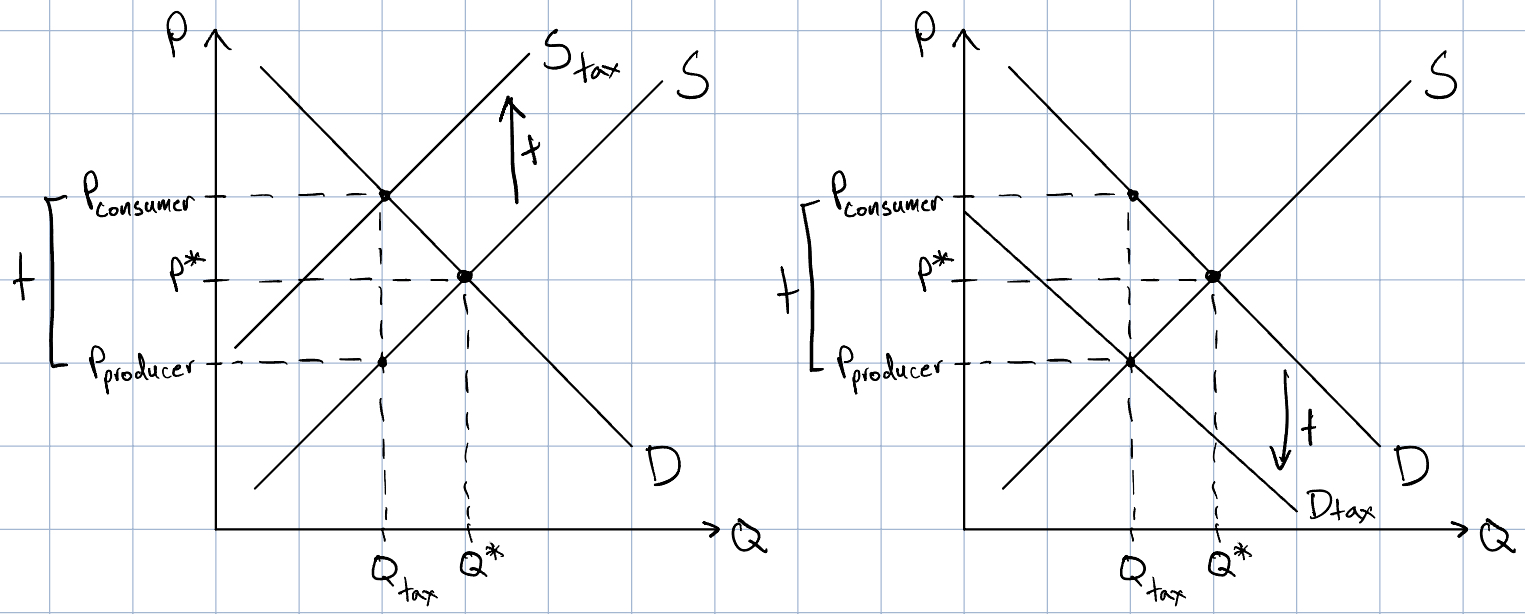
\includegraphics[width = \textwidth]{paa7a}
		\end{center}
		
	\item It would be more effective. If demand were more elastic, more people would find substitutes and stop buying gasoline when the tax increased the price consumers pay. As a result, the quantity traded would decrease by a greater amount.
		\begin{center}
		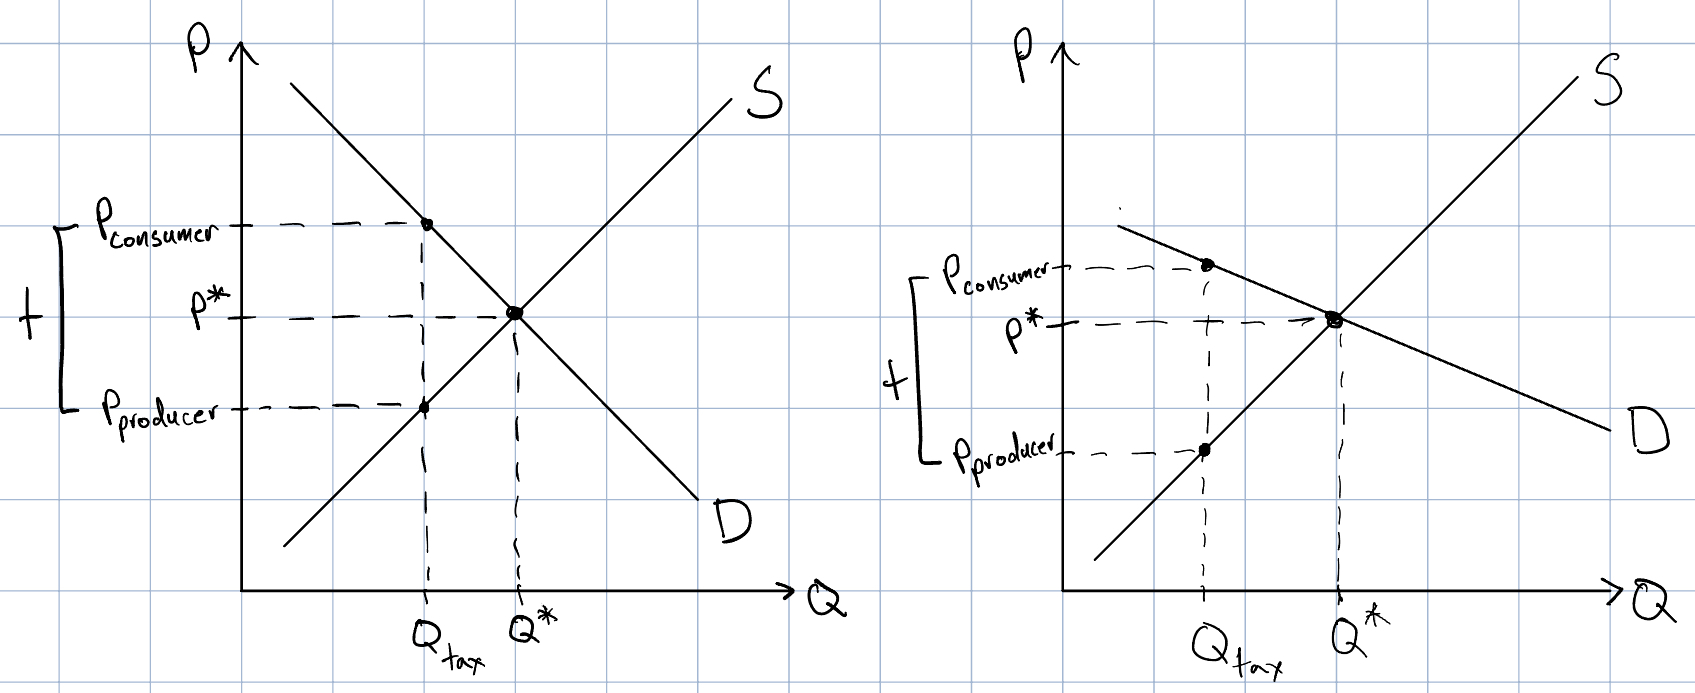
\includegraphics[width = \textwidth]{paa7b}
		\end{center}
		
	\item It depends on how much they value the decline in air pollution. They buy less and pay more for gas, so they're hurt in the gas market. That said, if they value clean air more than they value cheaper gas, they end up better off.
	
	\item It depends on how much they value the decline in air pollution. They sell less gas and take home a lower price than before, so they're hurt in the gas market. That said, if they value clean air more than they value better gas sales, they end up better off.
	
	\end{enumerate}

\end{enumerate}

\end{document}